\chapter{Fundamentos teóricos}

\section{Unidades Radiométricas}
Se conoce como radiometría al estudio de las radiaciones electromagneticas. Ya que la luz visible es una onda electromagnetica los algoritmos de renderizado que buscan el realismo se fundamentan sobre conceptos radiométricos. Por ello en esta sección haremos una pequeña introducción sobre algunos conceptos básicos que nos permitiran entender mejor los algoritmos de iluminación global.  
\subsection{Flujo}

El flujo radiometrico mide la cantidad de energia radiante por unidad de tiempo. Sus unidades son Watts o Joules/segundo.

\begin{equation}
\Phi = \frac{dQ(t)}{dt}
\end{equation}

\subsection{Irradiancia}
La irradiancia representa el flujo incidente en una superficie y se mide como el flujo radiante por unidad de area y sus unidades son de $W/m^2$ 

\begin{equation}
E = \frac{d\Phi}{dA}
\end{equation}

\clearpage

\subsection{Angulo solido}
El angulo solido no es una unidad radiométrica en si mismo pero es un concepto geométrico necesario para poder explicar otros conceptos radiométricos además de otros apartados del presente trabajo.

Podemos entender el concepto de angulo solido como la extension del angulo a las tres dimensiones.
\begin{figure}[h]
\centering
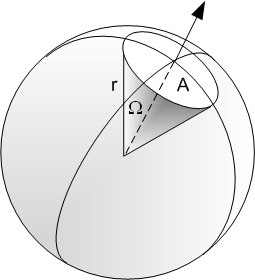
\includegraphics[width=2in]{Solid_Angle.png}
\caption{Definición de angulo solido \cite{Haade}}
\end{figure}

El angulo solido se mide como el área proyectada sobre una esfera de radio unitario. Sus unidades son adimensionales y son llamadas stereorradianes $[sr]$.
\begin{equation}
\Omega = \frac{A}{r^2}
\end{equation}


Usando coordenadas esféricas $\Theta = (\phi , \theta )$ podemos definir el angulo solido diferencial como:

\begin{equation}
d \omega _ \Theta = \sin \theta d \theta d \phi
\end{equation}

Informalmente resulta sencillo entender el angulo solido si pensamos en \emph{cuan grande se ve un objeto}. Supongamos una superficie perpendicular a la dirección de visión del observador: si este objeto esta muy cerca, diremos que subtiende un angulo solido mayor que la misma superficie a una mayor distancia en la misma dirección.

\clearpage

\subsection{Radiancia}

La radiancia, también llamada intensidad por algunos autores \cite{Kajiya1986, Immel1986}, es probablemente la unidad radiometrica mas importante en lo que concierne al presente trabajo.

Esta unidad mide la irradiancia por unidad de angulo solido.

\begin{equation}
L = \frac{dE}{d\omega} = \frac{d^2\Phi}{d\omega dA\cos \theta} 
\end{equation}


\clearpage

\section{BRDF}

La función de distribución de reflectancia bidireccional (de ahora en adelante BRDF, por sus siglas en inglés), definida por primera vez por \cite{Nicodemus1965} Nicodemus (1965), es un función que define la respuesta a la luz de una superficie opaca, tomando como parámetros dos vectores unitarios que definen las direcciones de entrada y salida de la luz. Más formalmente, la BRDF mide la relación entre la radiancia diferencial reflejada en la dirección de salida y la irradiancia diferencial entrante en el ángulo sólido diferencial alrededor del vector de entrada

\begin{equation}
f(x, l, v)=\frac{dL(x \to v)}{dE(x \gets l)} 
\end{equation}

donde $l$ es el vector unitario que apunta en la dirección opuesta a la de entrada de la luz y $v$ es el vector unitario que apunta en la dirección de salida de la luz.

La BRDF solo esta definida para vectores $l$ y $v$ tales que $n \cdot v > 0, n \cdot l > 0$, siendo $n$ la normal de la superficie.

\begin{figure}[h]
\centering
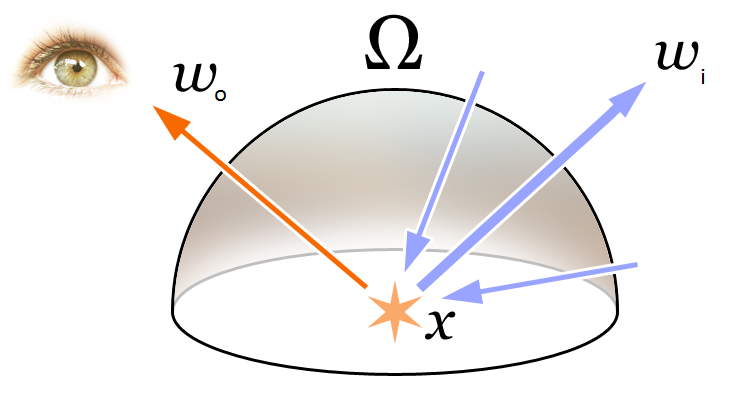
\includegraphics[scale=0.5]{Rendering_eq.png}
\caption{BRDF $l = \omega_i, v = \omega_o$ }
\end{figure}


Para obtener la radiancia total reflejada en un punto $x$ en la dirección saliente $v$ es necesario integrar sobre el angulo solido en el dominio de la hemiesfera centrada en $x$.

\begin{equation}
\label{eq:radiance_integral}
L _ o = \int_{\Omega_x} f(x, l, v) L_i(l) (l \cdot n) d\omega_i 
\end{equation}

\clearpage

\subsection{Propiedades de la BRDF}

Una BRDF debe cumplir ciertas propiedades para que sea físicamente plausible.
En primer lugar debe cumplir la ley de conservación de la energía. En el caso que nos ocupa esto significa que una superficie puede absorber luz, transformándola en calor, o puede reflejarla pero en ningún caso puede reflejar mas energía lumínica que la que recibe.

\begin{equation}
\forall l, \int_{\Omega_x} f(x,l,v) (n \cdot v) d\omega_o \leq 1
\end{equation}

En términos informales esta ecuación significa que la integral de toda la luz reflejada debido a un rayo de luz entrante nunca podrá ser superior a la luz entrante por ese rayo.

\medskip
Además también debe cumplir el \emph{principio de reciprocidad de Helmholtz}, esto significa que si intercambiamos los vectores $l$ y $v$ su valor se mantiene. Este hecho cobra sentido si pensamos que la BRDF es una característica intrínseca de cada material y que al intercambiar los vectores $v$ y $l$ el angulo entre ellos sigue siendo el mismo.

\begin{equation}
f(x, l, v) = f(x, v, l)
\end{equation} 


\clearpage

\section{Ecuación de renderizado}

La ecuación de renderizado fue desarrollada en los años 80 simultaneamente y de forma independiente por distintos autores \cite{Kajiya1986, Immel1986}. Se trata de una ecuación integral que unifica y formaliza los distintos algoritmos de renderizado, ya que hasta ese momento no existía un marco de trabajo teórico común.

\medskip
Existen varias versiones de esta ecuación segun el autor que la use que, en general, se pueden clasificar en dos tipos: las que integran sobre la hemiesfera, que se corresponde con la ecuacion propuesta por Immel y las que integran sobre la union de las superficies de la escena, que es la version propuesta por Kajiya.
\medskip

Consideremos la ecuación \ref{eq:radiance_integral}  y consideremos que además de dispersar luz una superficie también puede emitir luz, siendo $L_e$ la radiancia de la luz emitida, entonces tenemos la ecuación de renderizado.

\begin{equation}
L _ o = L_e + \int_{\Omega_x} f(x, l, v) L_i(l) (l \cdot n) d\omega_i 
\end{equation}




Donde I(x,x’) es la intensidad de la luz que llega del punto x’ al punto x, (x,x') es la intensidad de la luz emitida en el punto x’ hacia el punto x. (x,x',x'') es una función de distribución que determina qué proporción de la luz incidente en x’ proveniente de x’’ es rebotada hacia x. Esta función depende de las características de cada material y es comúnmente conocida como BRDF de sus siglas en inglés Bidirectional Reflectance Distribution Function.

El dominio de la integral, S, es la unión de todas las superficies de la escena S=Si
g(x,x’) es un término geométrico que determina la visibilidad entre los puntos x, x’.

A primera vista esta ecuación puede parecer imponente pero si nos olvidamos por un momento de los formalismos matemáticos y nos centramos en su significado, lo que viene a decir es que la luz que llega al punto x en la dirección x'x es igual a la luz emitida en el punto x’ en la dirección x'x más la integral de toda la luz que llega al punto x’ y es dispersada en la dirección x'x.

Lo significativo de esta ecuación es que resulta muy intuitivo derivar algoritmos de renderizado de la misma: se evalúa para cada punto a pintar y se evalúa I(x’, x’’) recursivamente hasta que se cumpla determinada condición.

\clearpage

\section{El método de montecarlo}

El método de montecarlo se trata de un método de integración numérico para integrales definidas sobre un dominio de dimension arbitraria, del tipo:
\begin{equation}
I = \int_D f(x)dx , D \subseteq \mathbb{R}^m
\end{equation}

Sabemos que la esperanza de una función continua se define como la integral de la función por la probabilidad de $x$. Y que podemos estimar la esperanza calculando la media de los valores que toma la función en puntos aleatorios escogidos independientemente y con la misma distribución.

\begin{equation}
E(f(x)) = \int f(x)p(x)dx \approx \frac{1}{N} \sum _{i=1} ^N f(x_i) 
\end{equation}


El método de montecarlo se basa en este hecho para estimar el valor de una integral definida tomando muestras aleatorias sobre el dominio $x_1, x_2, ..., x_n \in D$ y aplicando:

\begin{equation}
\label{eq:montecarlo}
I = \int_D f(x)dx \approx \frac{1}{N} \sum _{i=1} ^N \frac{f(x_i)}{p(x_i)} 
\end{equation}

Siendo $p(x_i)$ la probabilidad de tomar una muestra $x_i$ concreta de entre todas las posibles en el dominio $D$. En el caso de tomar las muestras sobre una distribución uniforme:

\begin{equation}
p(x_i) = \frac{1}{\int _D dx}
\end{equation}

\begin{equation}
I \approx \frac{\int _D dx}{N} \sum_{i=1} ^N f(x_i)
\end{equation}

El error en una estimación de este tipo se reduce a medida que $N$ crece.
\clearpage

\subsection{Muestreo de importancia}
    
Otra forma de reducir el error a parte de tomar mas muestras es tomarlas de forma mas inteligente. Anteriormente hemos supuesto que tomamos las muestras de una distribución uniforme sobre el dominio pero el método de montecarlo no impone ninguna limitación en este aspecto. Lo que implica que podemos tomar las muestras de otro tipo de distribuciones que sean mas apropiadas para cada caso. Por ejemplo tomando mas muestras en aquellas partes del dominio de integración que sean mas interesantes o importantes para nuestros propósitos.

\medskip

Para ello basta con tomar las muestras $x_1, x_2, ..., x_n$ según la distribución usada y substituir $p(x_i)$ en la ecuación \ref{eq:montecarlo} por la probabilidad correspondiente.

\subsection{Muestreo estratificado}


